\section{Performance Characterization of Sampling Systems}

\paragraph{a)}

According to the IEEE Standard the test methods for SINAD, SFDR and SINAD were implemented.
The calculation was quite straightforward and can seen in the matlab file PC\_ADC.m.

\paragraph{b)}

The plots of the different performance measures can be seen in Figure \ref{fig:snrplots}.

You can see that The SFDR stays almost constant over frequency.
The SFDR is calculated by dividing the signal amplitude by the biggest component of noise
and distortion. I observed some kind of distortion in the spectrum (Figure \ref{fig:spectrum}), which
is not in within the first 5 harmonics, but has the highest amplitude. By looking at plots of
different signals, I observed that the amplitude of this distortion stays almost the same over frequency.
Therefore, the SFDR only depends on the signal amplitude and the amplitude of that distortion
and stays almost constant.

The THD decreases very slightly over the frequency. This means that the harmonic distortions are decreasing.

The SINAD decreases over the frequency. Because the Signal stays the same and the THD is decreasing,
this means that the variance of the total noise process is increasing.
The noise in the signal is a superposition of different noise sources. One noise source is
the quantization  noise. The quantization noise is independent of the signal frequency. (look at
the formula for the quantization noise, derived in the lecture) Therefore, 
there must be another noise source which increases over the frequency.
I think that this increasing noise floor is caused by the aperture jitter.
The aperture jitter is a uncertainty of the time at which the signal is sampled. It can be 
modeled as a zero mean white noise. The variance of the noise of the sampled signal, caused
by the jitter depends on the variance of the time of the jitter and on the slope of the
signal. The slope of a sinus increases with the frequency. Therefore the variance of this
noise process also increases with the frequency of the signal.



\begin{figure}[h!]
 \centering
 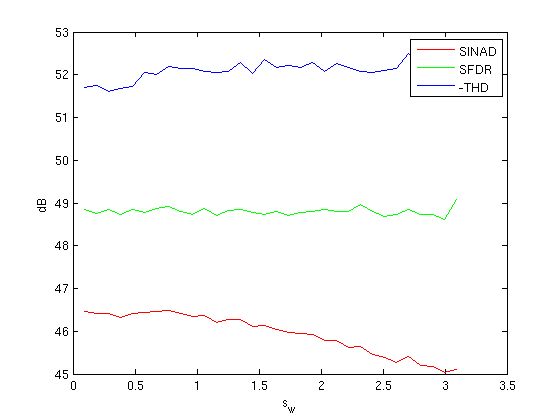
\includegraphics[width=\textwidth]{./pics/snrplots.png}
 % snrplots.png: 560x420 pixel, 90dpi, 15.81x11.85 cm, bb=0 0 448 336
 \caption{Plot of the different performance measures, SINAD, SFDR and THD over normalized frequency s\_W}
 \label{fig:snrplots}
\end{figure}


\begin{figure}[h!]
 \centering
 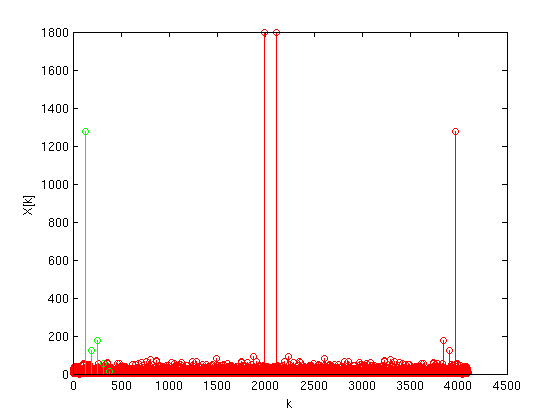
\includegraphics[width=\textwidth]{./pics/spectrum.png}
 % snrplots.png: 560x420 pixel, 90dpi, 15.81x11.85 cm, bb=0 0 448 336
 \caption{Plot of the spectrum of the first input signal, after the signal amplitude has been
 set to 0. What you can see in the plot is the spectrum of Noise and Distortion. The
 first 5 harmonics (aliasing component of the harmonics are not displayed in green) are marked as green.}
 \label{fig:spectrum}
\end{figure}


